\documentclass[12pt,oneside,a4paper]{article}

\pdfminorversion 4

\usepackage[margin=1in]{geometry}
\usepackage[toc,page]{appendix}
\usepackage{amsmath,amsfonts,amssymb}
\usepackage{graphicx, wrapfig}
\usepackage{color}
\usepackage{float}
\usepackage{tabularx,colortbl}

\usepackage{amsthm}

\usepackage[font=footnotesize]{caption}
\usepackage{subcaption}

\usepackage{fancyhdr}
\pagestyle{fancy}
\lhead{PHY 905 Project 1}
\rhead{Nicholas Miller}

% -------------------------------------------------

\renewcommand{\arraystretch}{1.25} 
\renewcommand{\baselinestretch}{1.0}

\begin{document}

\section{Theory}

\subsection{Ising Model}

The Ising model is a theoretical approximation of ferromagnetism.  It consists of discrete variables which, in our case, represent atomic spins in a two dimensional lattice.  These spin variables can take two values, shown in Eqn. (\ref{eq:spins}).
\begin{equation}
s_i =
\left\{
	\begin{array}{ll}
		+1, & \text{(spin up)} \\
		-1,  & \text{(spin down)}
	\end{array}
\right.
\label{eq:spins}
\end{equation}
Since the force between two atoms falls off as $r^{-3}$, the Hamiltonian is written as
\begin{equation}
E = -J\sum\limits_{\langle ij\rangle} s_i s_j - H\sum\limits_i s_i
\end{equation}
where $J=1$ is the interaction strength, $H$ is the magnetic field strength, and $\langle ij\rangle$ denotes summation over nearest neighbors.  For the rest of this report, the magnetic field strength will be $H=0$. 

At sufficiently low temperatures, the collection of atoms are permanently magnetized which is called ferromagnetic.  At sufficiently high temperatures, the atoms have zero magnetization and the temperature at which the phase transition between these two states is called the Curie Temperature $T_c$.

\subsection{Monte Carlo and the Metropolis Algorithm}

The magnetization of a collection of atomic spins are numerically calculated using the Monte Carlo method.  This involves choosing a random a subset of atom spins and averaging samples to compute observables.  For magnetization, the average value is given by Eqn. (\ref{eq:mag_avg}).
\begin{equation}
\langle M \rangle = \frac{\sum\limits_c M \exp\left(-E/kT\right)}{\sum\limits_c \exp\left(-E/kT\right)}
\label{eq:mag_avg}
\end{equation}
where the summation is over the total number of configurations $c = 2^{N_s}$ with $N_s$ independent spins.  For a reasonably small model of $N_s = 484$ (22 lattice points), the number of configurations exceeds the number of atoms in the universe, and most certainly exceeds the memory of the most powerful modern computer.  It is for this reason that the Metropolis Algorithm was invented -- to make possible the stochastic computation of the Ising model.

The Metropolis Algorithm is run for $N_xN_s$ iterations where $N_x$ is an integer:
\begin{itemize}
\item Given a specific configuration, flip a random spin $s_i\rightarrow -s_i$
\item Compute the change in energy $\Delta E$
	\begin{enumerate}
		\item Compute $w = \exp\left(-\Delta E / kT\right)$
		\item If $w \geq 1 (\Delta E \leq 0)$, accept flip
		\item else if $w > \left(\text{random number} \in \left[0,1\right]\right)$, accept flip
		\item else, reject flip
	\end{enumerate}
\end{itemize}
The main observable of the Ising model is the magnetization $M$ given by Eqn. (\ref{eq:magnetization}) which is averaged over the entire set of $N_x N_s$ configurations.
\begin{equation}
M = \sum\limits_i s_i
\label{eq:magnetization}
\end{equation}

\section{Some Coding Tricks}

\subsection{Precomputing Boltzmann Factors}



Computing the change in energy $\Delta E$ can be costly, but one way to ease the computational burden is by noticing that it only takes ten different values.  Consider the sum of nearest neighbor spins $\sum\limits_{i,nn}s_i$.  This summation can only be $\sum\limits_{i,nn}s_i \in \lbrace-4, -2, 0, 2, 4\rbrace$ and multiplying by the $j^\text{th}$ lattice point's spin $s_j$ gives two sets of spins $\sum\limits_{i,nn}s_i$ which are equal and opposite in sign.  Therefore the set of ten Boltzmann factors can be precomputed for a given temperature and accessed from memory during the Metropolis loop.

\subsection{Periodic Boundary Conditions}

To implement periodic boundary conditions, the edges of the two-dimensional lattice must be connected.  For instance, if the energy is computed at the $(i,j) = (1,1)$ site (top left corner), then the $(i-1, j)$ location must be mapped to $(N_i, j)$.  This can be accomplished with the modulo function in Python.  Given a $N_i \times N_j$ Python array (index starts at 0 in Python), the $(i-1, j)$ location is called as $( (i-1)\%N_i, j)$.  When $i \in \left[1, N_i\right]$, $(i-1)\%N_i = i-1$.  When $i=0$, however, $(i-1)\%N_i = N_i$ and the end lattice points are mapped together.  The same is done for all edges of the lattice.

\begin{figure}[!h]
	\centering
	\includegraphics[width=0.8\textwidth]{../results/magnetization_10x10_10k.pdf}
	\caption{Magnetization over temperature of a $10\times10$ periodic lattice with a $N_x=10,000$ scale to the number of Metropolis iterations.}
	\label{fig:mag10x10}
\end{figure}

\section{Results}

For all results, Boltzmann's constant $k_B$ was set to unity.  The magnetization of a $10\times10$ periodic lattice with $N_x = 10,000$ is shown in Figure \ref{fig:mag10x10}.  In the range of the phase transition ($2 \leq T \leq 2.5$) the average magnetization oscillates rapidly, but the expected behavior of the magnetization is within the error bars given by the standard deviation.  

Figure \ref{fig:mag50x50} displays three configurations at different temperatures.  Each configuration is the final after $N_x N_s$ Metropolis steps.  The lattice was $50\times50$ in size, and each lattice point is represented by either a black pixel (spin up) or a white pixel (spin down).  The lowest temperature configuration displays almost fully spin up, the middle temperature (near the Curie temperature) shows some collections of spins, and the high temperature displays almost fully random spins.  This matches what is expected from the Ising model.
\begin{figure}[!h]
	\centering
	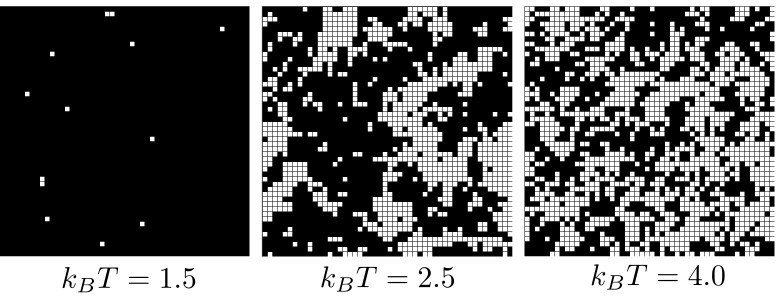
\includegraphics[width=\textwidth]{../results/50x50.pdf}
	\caption{Final configuration for three different temperatures.}
	\label{fig:mag50x50}
\end{figure}
\end{document}
